% !TeX spellcheck = en_US

\chapter{Software Design}
This chapter evaluates the possibility to use microservices for the WebUI components. It also describes the way, the user takes through the system. Finally the REST APIs consumed by the WebUI are described.



\section{Microservices for the WebUI}
\label{sec:MS_for_WebUI}
The MARS Websuite has been transfered into a mircroservice architecture. Backend services communicate via REST instead of local system calls. While this works very well for the backend, frontend components behave much different.\\
The code of a backend service is executed in an environment defined by the provider of the application, while the frontend is delivered to the user and executed by his browser.


\subsection{Constraints}
The bearing mentioned above, brings certain restrictions which are for technical and security reason. The following constraints have to be considered.

\subsubsection{Cross-origin issue}
Cross-origin requests are API calls to an IP or port other than the one, that provided the original webpage. These kind of requests can reveal confidential information stored in the session or a cookie inside the browser to a third party.\\
Therefore modern browsers implement the \textit{same-origin policy} as specified in the \textit{RFC 6454 -- The Web Origin Concept} by \cite{barth2011web}, which blocks cross-origin requests.\\
Write access to cross-origin locations and certain tags are excluded from the restrictions, among them are \textit{<a>} \textit{<img>}, \textit{<video>}, \textit{<iframe>} and \textit{@font-face}. While not reccomended, it is also possible to deactivate the strict origin policy.

\subsubsection{Only one initial URL}
The user opens a website by typing an URL to the address-bar of his browser. This implies, that one endpoint needs to deliver the whole side. This page has to either load other parts dynamically, or has to aggregate the content of the other frontend microservices in the backend, before it is delivered to the browser.

\subsubsection{tightly coupled}
As mentioned in Section \ref{sec:angularjs}, the Websuite consists of an AngularJS single-page application. This implies, that it is indeed a single page, that uses routing to redirect from different pages. That being said, it is not possible to fetch single pages from another service during runtime.

\subsection{possible Solutions}
The cross-origin issue is quite common for any site that has more than one backend to communicate with. The solution is, to deliver the whole page and all the consumed REST endpoints over a reverse proxy. The Websuite does this via Zuul.\\
The harder part is to split up the frontend. To do this, there are a few options.

\subsubsection{AJAX}
On this approach an empty page is delivered to the user. Afterwards, the client dynamically loads the required sections of a page from different locations, using asynchronous JavaScript calls.\\
This approach no backend configuration, since the frontend handles the composition, but will resolve in many calls to the backend, which might impact performance.

\subsubsection{iFrames}
This is similar to the AJAX approach, but uses iFrames to embed the fragments into the page. The content of the page can not be cached, which will increase the performance hazard.\\
Also the content can not control the size of the frame and is not able to communicate with other frames. While workarounds exist, iFrames are a relict from the 90s with the exception of a few use-cases.

\subsubsection{Edge Side Includes}
Edge Side Includes (ESI) is a server-side markup language. It is capable of dynamically adding fragments of a page together to one page. As this generates substantial CPU load on the server, a Cache like Varnish is used to make it usable in production. Varnish is one of the few options that supports ESI, which is why, it is why it is the most common choice for ESI.\\
This approach requires a high amount of configuration, to make the Varnish work properly. It includes setting the time-to-live (TTL) for the fragments on the page, based on the content.\\
The way ESI includes resource files like JavaScript, HTML and CSS can not guaranty consistency between the cached versions. This mean that an update in the HTML and JS might deliver the new HTML without the JS, which leads to errors in production.

\subsubsection{Server Side Includes}
Server Side Includes (SSI) is a server-side scripting language supported by the common web-servers like Apache and NGINX, which makes it more accessible than ESI. Caching is mandatory, like it is for ESI, but the lock-in to Varnish does not exist.\\
Unlike ESI, SSI can guarantee the consistency between cached resource files, which makes it a more appealing solution.

%\subsubsection{Compoxure}
%Compoxure is a middleware that tries to serve as an alternative to ESI and SSI with reduced setup afford. It also allows for a more fine-tuned caching of resources. 

\subsubsection{Web Components}
Web Components are a set of features that are being developed as a W3C standard for UI composition.
\begin{itemize}
	\item \textbf{Custom Elements:} Allows creation of custom HTML tags, like Angular's directives.
	\item \textbf{Shadow DOM:} Are elements, located outside the DOM and allow encapsulation of JS or CSS.
	\item \textbf{HTML Import:} Allows including reusable HTML snippets.
	\item \textbf{HTML Template:} Allows to define templates, that are evaluated once they are used. Resources are fetched, once needed.
\end{itemize}

Web Components seem like a promising development towards native support for decoupled frontends. However, the components are not fully supported by the common browsers jet.


\subsection{general considerations}
Splitting frontends into small services seems like an interesting thought. However, each of the approaches has downsides and that does not even consider some shared issues.\\
Modern frontends require a substantial amount of other code to function. These dependencies are all transfered to the client's browser prior to execution. This requires very strict control of the dependencies to prevent additional load or incompatibilities.\\
For the reasons mentioned above, most cases of composed frontends take advantage of the \textit{Backend for Frontend (BFF)} pattern, which keeps dependencies and code in the frontend to a minimum and builds backends directly tailored to the frontend.\\
The MARS Websuite is not build this way. The backend services provide data and the WebUI contains a lot of logic to prepare and convert data. The AngularJS framework and the other dependencies are not considered small either.\\


\subsection{conclusion}
Composing a frontend into multiple parts, requires to consider many aspects. While there are solutions, the afford is not to be underestimated with the currently available technologies. This being said, the effort is only worth it, for very big applications with many developers involved.\\
Moving the MARS WebUI to such a technology would mean to completely rebuild it and reworking the backend services. While the afford would be substantial, it is questionable, if the result would be an improvement. This is due to the fact that additional complexity always introduces potential failures.


\section{Work-flow}
% Way of the user through the system

\begin{figure}[H]
	\centering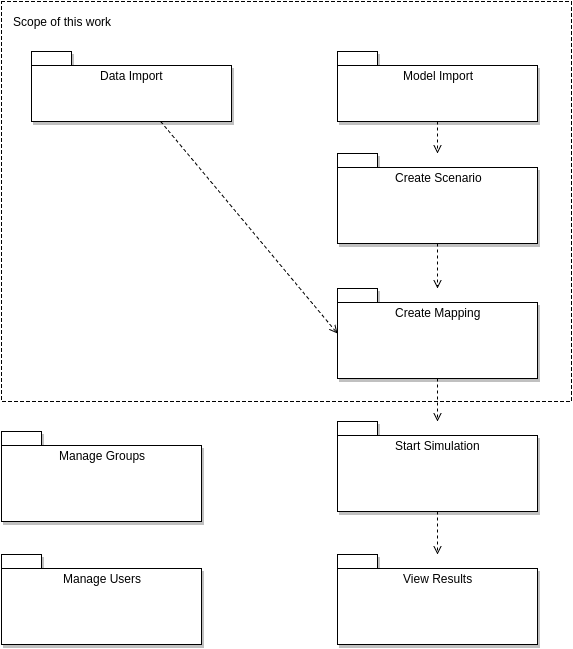
\includegraphics[width=.7\textwidth]{res/Dependency-workflow}
	\caption{Dependency work-flow}
	\label{fig:dependency-workflow}
\end{figure}



\section{Interface Description}
% rest Aufrufe